\documentclass[oneside]{memoir}
\usepackage{fontspec}
\usepackage[hidelinks]{hyperref}
\usepackage{microtype}
\usepackage{amsmath}
\usepackage{amssymb}
\usepackage{bm}
\usepackage{xcolor}
\usepackage{booktabs}
\usepackage{graphicx}
\usepackage[euler-digits,euler-hat-accent]{eulervm}

\setlrmarginsandblock{3.5cm}{2.5cm}{*}
\setulmarginsandblock{2.5cm}{*}{1}
\checkandfixthelayout

\definecolor{ACCgreen}{HTML}{28A745}

\newcommand\ddfrac[2]{\frac{\displaystyle #1}{\displaystyle #2}}

\setmainfont{TeX Gyre Pagella}

\usepackage{xcolor}
\hypersetup{
    colorlinks,
    linkcolor={red!50!black},
    citecolor={blue!50!black},
    urlcolor={blue!80!black}
}

\def\chapterheadstart{}

\begin{document}

\chapter*{Atomic Charge Calculator \textcolor{ACCgreen}{II}}
Atomic Charge Calculator II (ACC II) is a web application providing a user interface for the computation of partial atomic charges. The application consists of three pages – main introductory one, computation setup, and visualization of the results.

\section*{Main page}
The main page offers a possibility to upload your own structure (in one of the supported formats: SDF, PDB, Mol2, and mmCIF).

Clicking on "Compute charges" button will automatically select the most appropriate method, executes the computation and redirects to the Results page. "Setup computation" can be used for manually selecting the method and parameters.

\begin{center}
    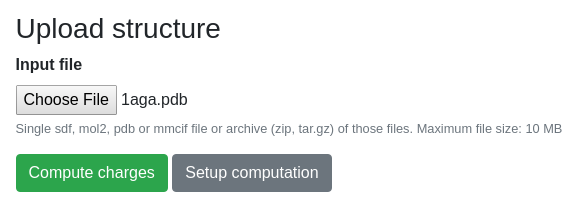
\includegraphics[width=.5\linewidth]{images/upload.png}
\end{center}

\subsection*{Input files notes}
Input file can be zipped. A size of input file is limited to 10 MB.
\begin{description}
\item[PDB, mmCIF] When file contains multiple models, only the first one is used for computation. All atoms (including HETATM) atoms are considered.
\item[SDF] Both MOL V2000 and V3000 are supported.
\end{description}

\subsection*{How to set input charge values}

Formal charges, if present, are read from an input file as well. Their sum is used as a total molecular charge, which is used by some methods (ABEEM, EEM, EQeq, Eqeq+C, QEq, SFKEEM, SMP/QEq, TSEF).

Specification of input formal charges differs among supported file formats, ACC II reads the following:

\begin{description}
\item[SDF] \texttt{M  CHG} lines for MOL V2000; for MOL V3000 the charge is read from \texttt{CHG} property of \texttt{ATOM} records. See the \href{https://www.daylight.com/meetings/mug05/Kappler/ctfile.pdf}{documentation} of the format.
\item[PDB*] Columns 79-80 of the \href{http://www.wwpdb.org/documentation/file-format-content/format33/sect9.html#ATOM}{\texttt{ATOM} record}.
\item[mmCIF*] \href{http://mmcif.wwpdb.org/dictionaries/mmcif_pdbx_v50.dic/Items/_atom_site.pdbx_formal_charge.html}{\texttt{\_atom\_site.pdbx\_formal\_charge}} record; or \href{http://mmcif.wwpdb.org/dictionaries/mmcif_pdbx_v50.dic/Items/_chem_comp.pdbx_formal_charge.html}{\texttt{\_chem\_comp.pdbx\_formal\_charge}} record in case of chemical components.
\item[Mol2] Not supported.
\end{description}

\textbf{*} Read using the \href{https://project-gemmi.github.io/}{GEMMI} library.

\section*{Computation settings}
Based on the molecules provided (in all files), methods and parameters that are suitable for all structures are displayed. The parameter set is suitable for a given input if it covers all the atomic types contained in input files. A method is suitable if it has at least one suitable set of parameters; or uses no parameters. Additionally, some methods (namely ABEEM, DelRe, DENR, KCM, MGC) might be omitted if the input contains at least one big molecule, i.e., having over 20,000 atoms.

Automatic selection works in a same manner. After initial filtering described above, 3D methods are preferred over the 2D ones. When input contains protein structures, parameters for proteins are used (this is the case for EEM having the most parameters to choose from).

\begin{center}
    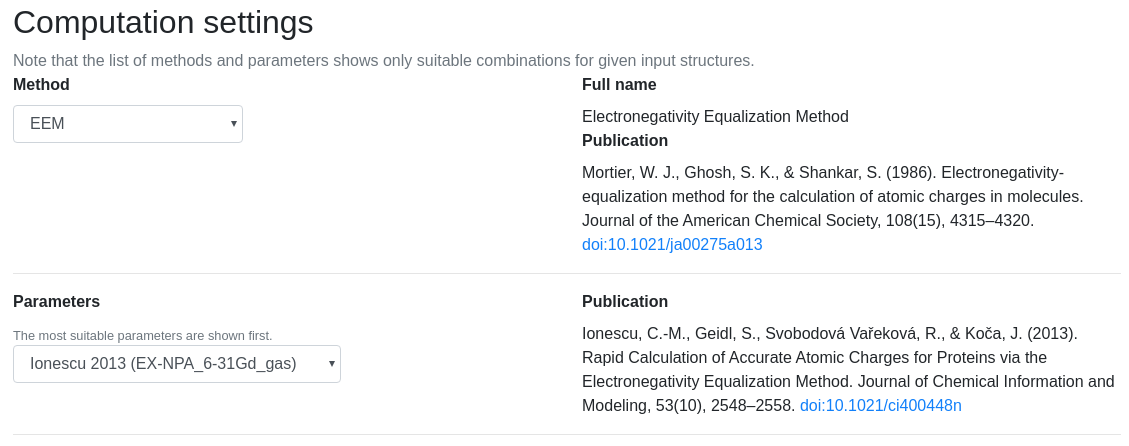
\includegraphics[width=.9\linewidth]{images/settings.png}
\end{center}

All the methods and parameters have direct links to the original publications. The theoretical background of the methods is summarized in the \href{https://acc2.ncbr.muni.cz/static/methods.pdf}{standalone document}. For easy identification, the name of the parameters used in a publication is enclosed in the brackets.

\section*{Results}
The final page features the visualization of the charges and the possibility to download calculated charges. At the top, it states which method and parameters were used (useful when the automatic selection was used).

When multiple structures were provided, the user can switch between those using the select box.

\begin{center}
    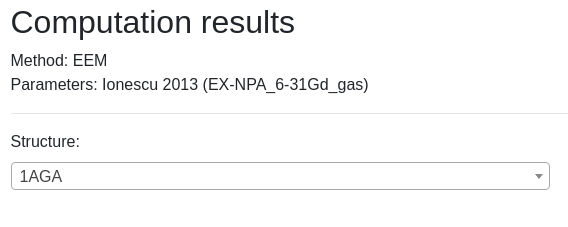
\includegraphics[width=.5\linewidth]{images/select.png}
\end{center}

\subsection*{Visualization modes}
ACC II features fast LiteMol viewer to visualize calculated charges. There are three standard modes the user can select – balls-and-sticks, cartoon, and surface –  see example (1F16):

\begin{figure*}[h!]
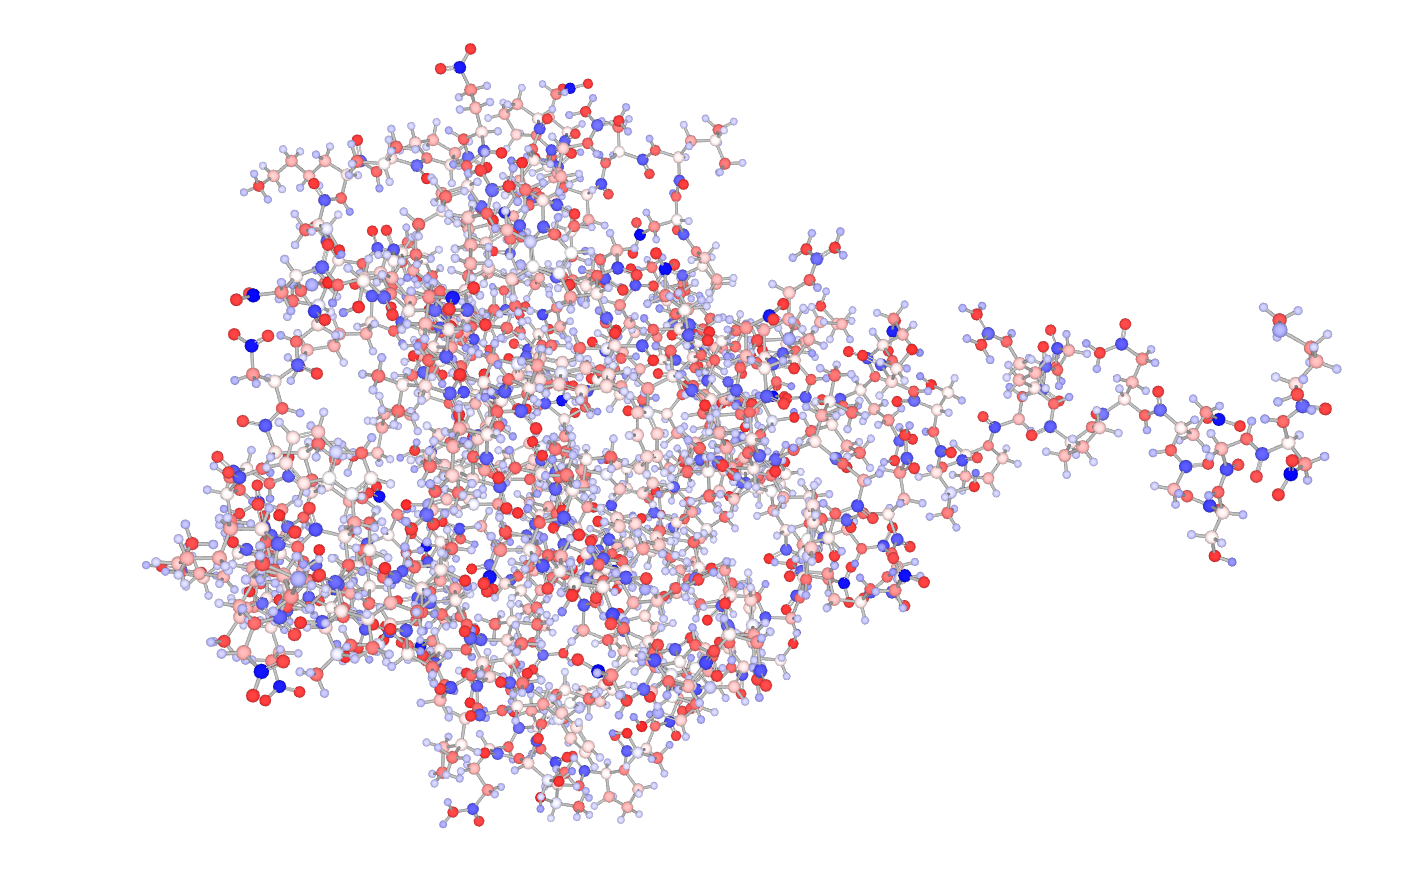
\includegraphics[width=.45\linewidth]{images/bas.png}
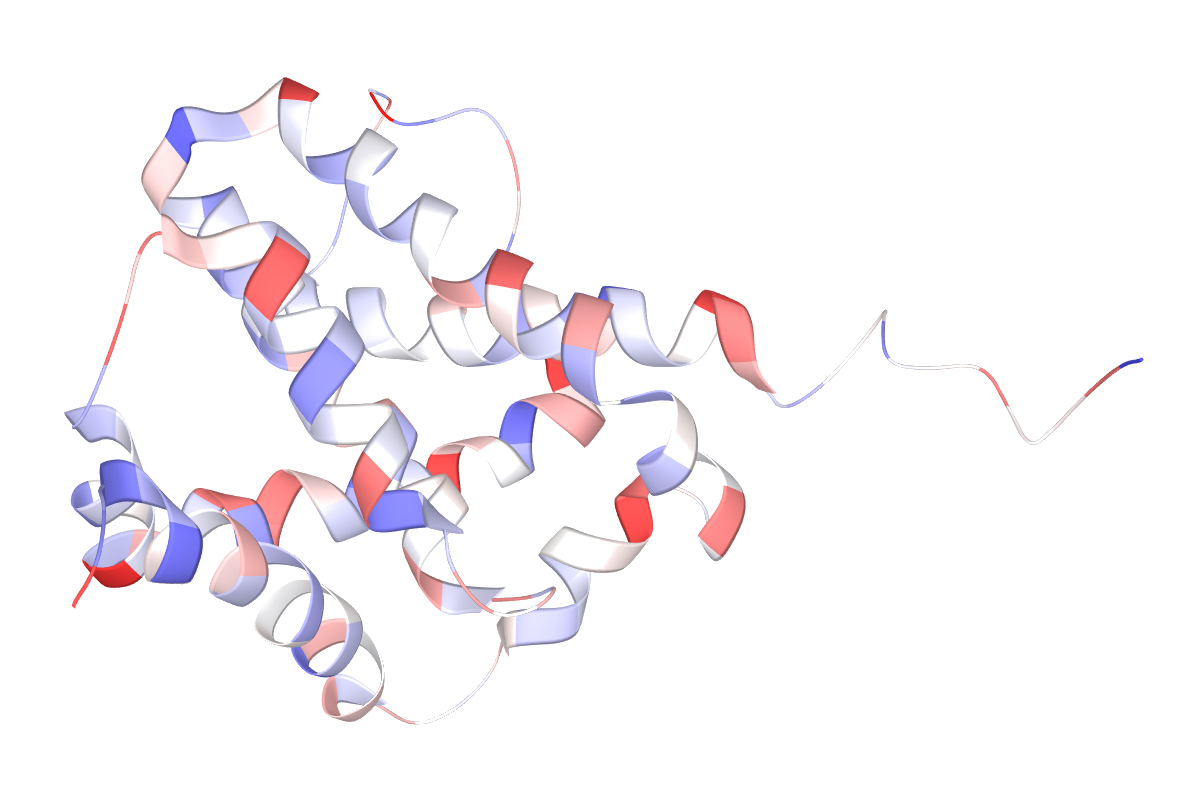
\includegraphics[width=.45\linewidth]{images/cartoon.png}
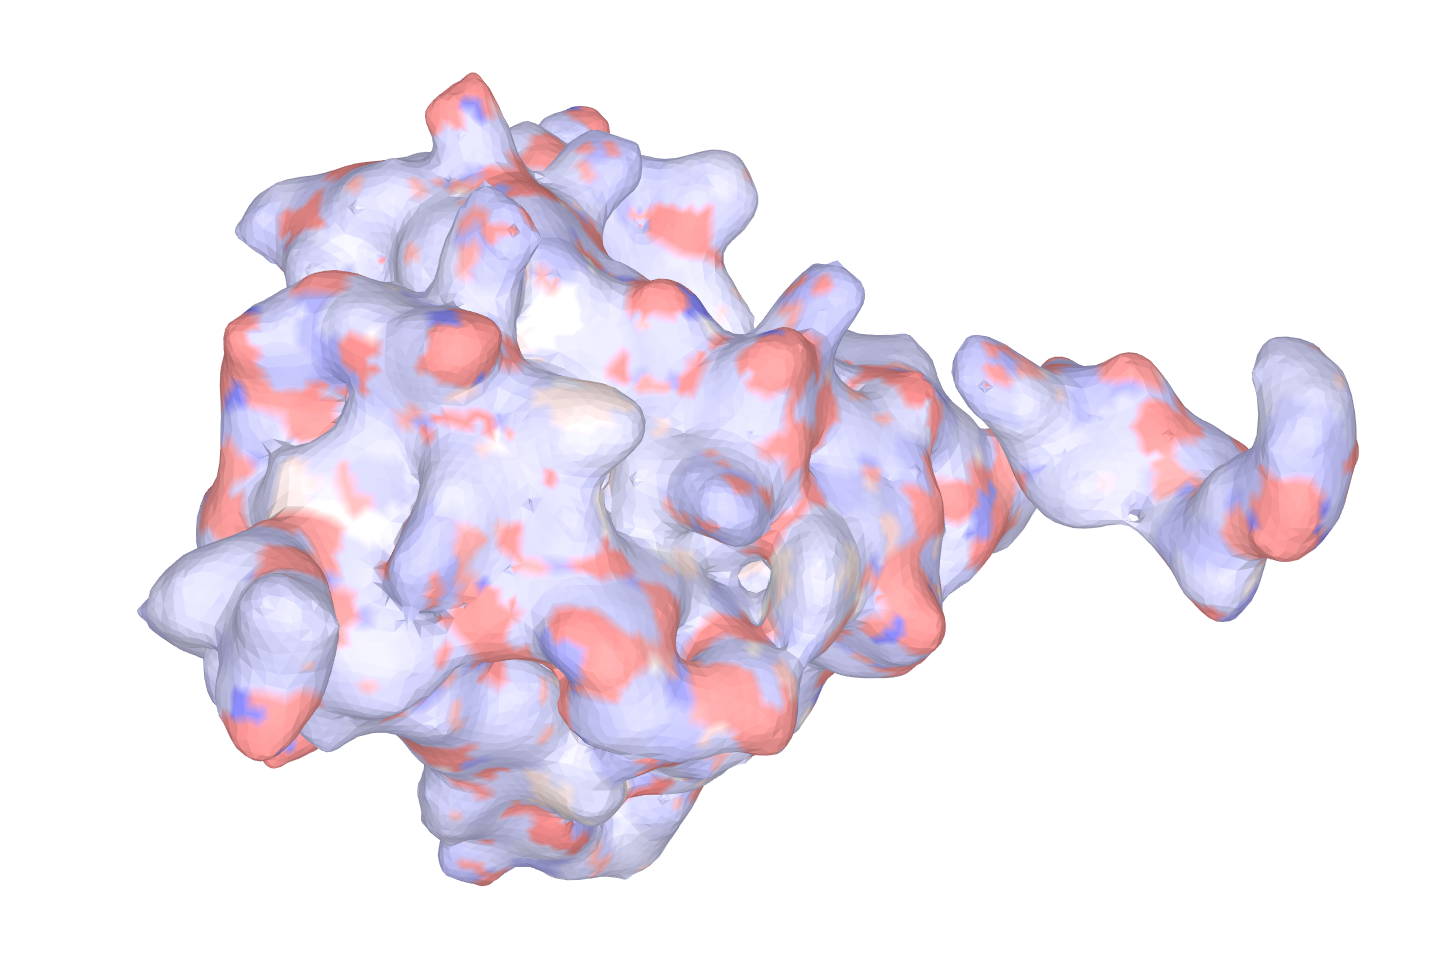
\includegraphics[width=.45\linewidth]{images/surface.png}
\end{figure*}

Default is determined from the structure itself.
Note that to visualize mmCIF files, they must contain \texttt{\_atom\_sites} category (chemical components won't work).

\subsection*{Coloring options}
Atoms are colored by charges by default – red for negative charges, blue for positive ones. When relative coloring is selected, the range for the colors is adjusted automatically based on the largest absolute value of a charge computed. To have comparable colors between different structures, absolute coloring should be used instead.

In cartoon mode, the color of individual residue is determined according to the sum of charges of all the comprised atoms. In surface mode, the point on the surface of the molecule is colored according to the nearest atom. Alternatively, coloring by charges can be disabled – colors are selected based on the elements.

\subsection*{Downloading data}
The charges are available in three formats – plain text, Mol2, and PQR. Plain text is present for all the inputs, PQR when input contains structures with chain specification (most likely protein) and Mol2 otherwise (small molecules).

\section*{Browser compatibility}

\begin{tabular}{llllll}
\toprule
OS & Version & Chrome & Firefox & Edge & Safari\\
\midrule
Linux & Fedora 31 & 80 & 73 & n/a & n/a\\
Windows & 10 (1909) & 80 & 73 & 44 & n/a\\
macOS & 10.14.6 & 80 & 74 & 80 & 12.1\\
\bottomrule

\end{tabular}

\section*{Bug reporting}
If you encounter an error, please send a report to \href{mailto:krab1k@mail.muni.cz}{krab1k@mail.muni.cz}. Thank you!

\end{document}
